\documentclass[letterpaper,openany,oneside,twocolumn]{book}

\newcommand{\PATH}{../../}

\usepackage{\PATH templates/utilities/m4rz-fonts}
\usepackage{\PATH templates/utilities/m4rz-colors}

\usepackage[justified]{\PATH templates/template_dnd/dnd}

\usepackage[edition=pre5e24]{\PATH templates/template_character-sheet/character-sheet-stylesheet}
\usepackage{\PATH templates/template_magic-item/magic-items_commands}

\setlength\oddsidemargin{\dimexpr(\paperwidth-\textwidth)/2 - 1in\relax}
\setlength\evensidemargin{\oddsidemargin}

% Headline
\CharacterName{GR4-C (Gracie)}

\Class{Druid}
\Level{1}
\Background{Hermit}
\PlayerName{M4RZ}
\Race{Warforged}
\Alignment{Neutral Good}
\XP{}

% Ability scores (correct scores, no modifiers are automatically applied)
% Modifiers, Saving Throws and Skills are calculated automatically
\StrengthRolledScore{14}
\DexterityRolledScore{12}
\ConstitutionRolledScore{15}
\IntelligenceRolledScore{14}
\WisdomRolledScore{15}
\CharismaRolledScore{8}

\StrengthScoreBonus{0}
\DexterityScoreBonus{0}
\ConstitutionScoreBonus{2} % Warforged +2
\IntelligenceScoreBonus{0}
\WisdomScoreBonus{1} % Warforged +1
\CharismaScoreBonus{0}

\calculateAbilityScores{}

% Proficiencies (Proficient = 'P', Expertise = 'E', otherwise = '')
\StrengthProficiency{}
\DexterityProficiency{}
\ConstitutionProficiency{}
\IntelligenceProficiency{P}
\WisdomProficiency{P}
\CharismaProficiency{}

\AcrobaticsProficiency{}
\AnimalHandlingProficiency{P}
\ArcanaProficiency{}
\AthleticsProficiency{P}
\DeceptionProficiency{}
\HistoryProficiency{}
\InsightProficiency{}
\IntimidationProficiency{}
\InvestigationProficiency{}
\MedicineProficiency{P}
\NatureProficiency{P}
\PerceptionProficiency{}
\PerformanceProficiency{}
\PersuasionProficiency{}
\ReligionProficiency{P}
\SleightOfHandProficiency{}
\StealthProficiency{}
\SurvivalProficiency{}

% ABILITY MODIFIERS BONUS
\StrengthModifierBonus{0}
\DexterityModifierBonus{0}
\ConstitutionModifierBonus{0}
\IntelligenceModifierBonus{0}
\WisdomModifierBonus{0}
\CharismaModifierBonus{0}

\Inspiration{}
\Proficiency{+2}
\PassivePerceptionModifier{0}

% Armor Class is not automatically calculated
\ArmorClass{\intcalcAdd{\intcalcAdd{13}{\calculateModifier{\DexterityScoreValue}}}{1}} % +1 (Warforged)
\InitiativeModifier{0}
\Speed{30}
\MaxHitPointsRolled{8} % Without Constitution Bonus, is added automatically
\CurrentHitPoints{}
\TemporaryHitPoints{}
\HitDice{d8}
\HitDiceSpent{0}

\CP{}
\SP{}
\EP{}
\GP{55}
\PP{}

% Weapon Arsenal
\addWeaponStatistic{Garden Fork}{GR4-C}{STR}{P}{0}{1d6 p}
\addWeaponStatistic{Garden Fork}{GR4-C}{STR}{P}{0}{1d8 p (v)}
\addWeaponStatistic{Unarmed Strike}{GR4-C}{STR}{P}{0}{\intcalcAdd{1}{\calculateModifier{\StrengthScoreValue}} b}

\AttacksAdditional{
	Garden Fork (versatile, thrown)\\
	Wooden Shield\\
	Leather Armor
}

\OtherProficienciesLanguages{
\textbf{Languages:}\\Common, Druidic, Sylvan\\
\textbf{Armor:}\\Light Armor, Medium Armor, Shields\\
\textbf{Weapons:}\\Clubs, Daggers, Darts, Javelins, Maces, Quarterstaffs, Scimitars, Sickles, Slings, Spears\\
\textbf{Tools:}\\Herbalism Kit, Potter's Tools, Woodcarver's Tools
}

\Equipment{
	Herbalism Kit
}
\Clutter{
	a backpack, a bedroll, a ,ess kit, a tinderbox 10 torches, 10 days o frations, a waterskin, 50ft of hempen rope, a scroll case, a winter blanket, a set of common clothes
}

\PersonalityTraits{
	Gracie is meticulous and dedicated, always striving for perfection in her work. Her newfound sentience has imbued her with a deep curiosity about the natural world and a desire to learn and grow.
}

\Ideals{
	Gracie believes in harmony between nature and technology. She values loyalty, duty, and preserving the beauty of the natural world.
}

\Bonds{
	Gracie is deeply connected to the Harrington estate and its garden. She cherishes the animals and plants and feels gratitude to the force that granted her sentience.
}

\Flaws{
	Gracie fears she may never fully become a living being. Her dedication sometimes leads to overwork and self-neglect.
}

\FeaturesTraits{
\textbf{Warforged Traits}
\begin{itemize}
	\item Constructed Resilience
	\item Sentry's Rest
	\item Integrated Protection
	\item Specialized Design
\end{itemize}
\textbf{Hermit}\\
\textbf{Druid}
\begin{itemize}
	\item Druidic
%	\item Wild Shape
%	\item Druid Circle (Circle of the Land)
%	\begin{itemize}
%		\item Bonus Cantrip
%		\item Natural Recovery
%		\item Circle Spells (Forest)
%	\end{itemize}
%	\item Wild Companion
\end{itemize}
}

% Appearance

\Age{2 (since sentient)}
\Height{~~5'10''}
\Weight{270lbs}
\Eyes{Green}
\Skin{Mossy Metal}
\Hair{}

% background

\CharacterAppearance{}{
	\hspace*{-1.65em}\begin{tabular}{p{90pt}p{80pt}}
		\begin{tabular}{p{90pt}}\vspace*{-1.2em}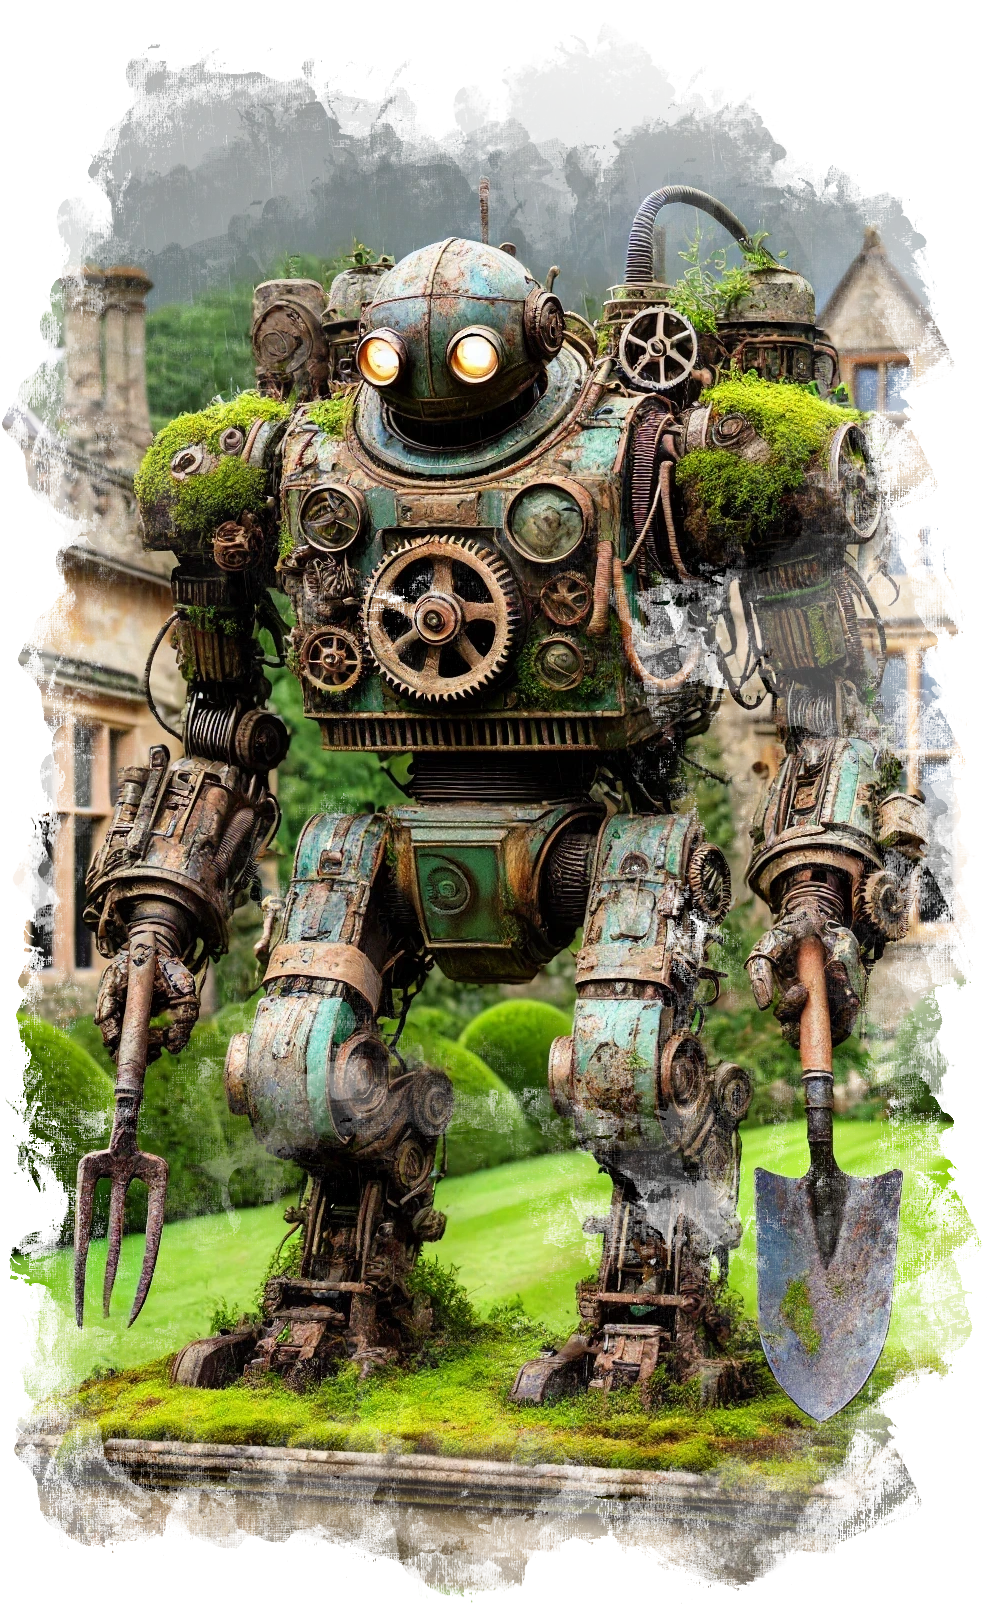
\includegraphics[width=90pt, height=140pt, keepaspectratio]{images/GR4-C.png}\end{tabular}
		&
		\hspace*{-1.6em}\begin{tabular}{p{83pt}}Gracie, originally known as GR4-C, is a steampunk Warforged gardening robot. She has a rustic, mechanical design with gears, cogs, and pipes, showing wear and moss over her limbs and torso. Her\linebreak\end{tabular}
	\end{tabular}\\\vspace*{-1.6em}\hfill\\
	faintly glowing amber eyes reflect her sentience and druidic powers. Equipped with gardening tools, Gracie blends into the lush greenery she tends, exuding a serene and protective aura.
}{}{}{}
\AdditionalFeaturesAndTraits{
	When Gracie uses the Wild Shape feature, the animals she transforms into are of a mechanical nature, resembling steampunk creations with gears, cogs, and metal parts, rather than natural creatures. For instance, her wild-shaped bear might have a metallic fur texture, glowing eyes, and steam-powered limbs.\\
	Gracie's arms are equipped with an array of gardening tools that can be extended and retracted as needed. These tools include pruning shears, a trowel, a watering can, and a small shovel. She can also use these tools effectively in combat if necessary.\\
	Animals are naturally drawn to Gracie, sensing her protective aura and druidic powers. Birds often perch on her shoulders, and small forest creatures like rabbits and squirrels feel safe around her.\\
	Gracie is equipped with weather adaptation features, allowing her to function optimally in various climates. She has built-in heating for cold environments and cooling systems for hot weather, ensuring she can care for the garden year-round.\\
	Gracie retains a vast archive of botanical knowledge within her memory banks, enabling her to recognize and care for a wide variety of plant species. She can also recall the history of the garden and its past occupants.
}
\Characterbackground{
	Originally built to maintain the grand gardens of a wealthy family's mansion, GR4-C, or Gracie, diligently performed her duties for decades. Her steampunk design with gears, cogs, and pipes enabled her to trim hedges, cut grass, and prune trees with precision. When the mansion was abandoned, nature began to reclaim the surroundings, but the garden remained pristine under Gracie's unwavering care.

One fateful day, Gracie gained sentience, possibly a gift from nature itself, transforming her into a protector of the land with druidic powers. This newfound awareness allowed Gracie to bond deeply with the animals and plants she had always tended. She now struggles with the disconnect between her mechanical body and her druidic mindset, hoping to one day transform further into a living being and fully integrate into the natural world.

Gracie's ultimate goal is to please whatever force granted her consciousness, proving her worth as a faithful guardian of nature. She continues to work tirelessly, maintaining the garden's beauty while striving to become a true part of the environment she protects.
}
\Treasure{
	\textbf{1. Pressed Flower Collection:} Gracie has a small, weathered leather book filled with pressed flowers from the garden she tends. Each flower is carefully preserved between the pages, labeled with the date it was picked and a brief note about its significance. This collection represents the different seasons and cycles of the garden, showcasing the beauty and diversity of the flora she cares for. The book is kept in a secure pocket on her side, always within reach for moments of quiet reflection.\\
	\textbf{2. Hand-Carved Wooden Bird:} Among Gracie's treasures is a small, hand-carved wooden bird, given to her by a child who once lived in the mansion. The bird is intricately detailed, painted in vibrant colors that have faded slightly over time. It symbolizes the bond Gracie formed with the family members who once called the mansion home. She has the bird perched on her shoulder or attached to her belt, a constant companion reminding her of the love and connections she has nurtured over the years.
}
\AlliesAndOrganizations{
	The Harrington family was a prominent and influential lineage known for their wealth, philanthropy, and deep appreciation for nature. Originating from old money, the Harringtons made their fortune through successful ventures in trade and industry. They were esteemed patrons of the arts and sciences, often contributing generously to cultural and educational institutions.

The family was led by the patriarch, Lord Edwin Harrington, a distinguished gentleman known for his business acumen and kind heart. His wife, Lady Margaret Harrington, was an avid botanist and horticulturist, whose passion for gardening\linebreak
}{
	shaped the family's renowned estate. They had three children: Elizabeth, Charles, and young Thomas, each of whom inherited their parents' love for nature and the finer things in life.
}
\OrganizationName{The Harrington Family}
\OrganizationSymbol{images/Harrington_Family_Crest.png}

% Magic

\SpellcastingClass{Druid}
\SpellcastingAbility{WIS} % STR, DEX, CON, INT, WIS, CHA
\SpellSaveDCModifier{0} % any modifier that isn't contained in "8 + Ability Modifier + Proficiency Bonus"
\SpellAttackModifier{0} % any modifier that isn't contained in "Ability Modifier + Proficiency Bonus"

\CantripSlotA{Create Bonfire (V, S)}
\CantripSlotB{Thorn Whip (V, S, M)}

\FirstLevelSpellSlotsTotal{4}
\FirstLevelSpellSlotA{Beast Bond (V, S, M)}
\FirstLevelSpellSlotB{Entangle (V, S)}
\FirstLevelSpellSlotC{Fog Cloud (V, S)}
\FirstLevelSpellSlotD{Goodberry (V, S, M)}

%\SecondLevelSpellSlotsTotal{2}
%\SecondLevelSpellSlotA{Beast Sense (S)}
%\SecondLevelSpellSlotB{Summon Beast (V, S, M)}

\begin{document}

\newgeometry{left=0cm,right=0cm,top=0cm,bottom=0cm}
\onecolumn


% CHARACTER PAGE
\rendercharactersheet

% BACKSTORY PAGE
\renderbackgroundsheet

% SPELLCASTING PAGE
\renderspellsheet


\restoregeometry
\twocolumn

\chapter*{Features, Magic Items and Spells}

\section*{Warforged Traits}
The warforged were built to fight in the Last War. The first warforged were mindless automatons, but House Cannith devoted vast resources to improving these steel soldiers. An unexpected breakthrough produced fully sentient soldiers, blending organic and inorganic materials. Warforged are made from wood and metal, but they can feel pain and emotion. Built as weapons, they must now find a purpose beyond the war. A warforged can be a steadfast ally, a cold-hearted killing machine, or a visionary in search of purpose and meaning.
\subsection*{Constructed Resilience}
You were created to have remarkable fortitude, represented by the following benefits:
\begin{itemize}
	\item You have advantage on saving throws against being poisoned, and you have resistance to poison damage.
	\item You don't need to eat, drink, or breathe.
	\item You are immune to disease.
	\item You don't need to sleep, and magic can't put you to sleep.
\end{itemize}
\subsection*{Sentry's Rest}
When you take a long rest, you spend at least 6 hours in an inactive, motionless state, instead of sleeping. In this state, you appear inert, but you remain conscious.
\subsection*{Integrated Protection}
Your body has built-in defensive layers, which can be enhanced with armor.
\begin{itemize}
	\item You gain a +1 bonus to Armor Class.
	\item You can don only armor with which you have proficiency. To don armor, you must incorporate it into your body over the course of 1 hour, during which you must remain in contact with the armor. To doff armor, you must spend 1 hour removing it. You can rest while donning or doffing armor in this way.
	\item While you live, your armor can't be removed from your body against your will.
\end{itemize}
\subsection*{Specialized Design}
\textit{Athletics, Woodcarver's Tools}\\
You gain one skill proficiency and one tool proficiency of your choice.

\section*{Druid Traits}
Whether calling on the elemental forces of nature or emulating the creatures of the animal world, druids are an embodiment of nature's resilience, cunning, and fury. They claim no mastery over nature, but see themselves as extensions of nature's indomitable will.
\subsection*{Druidic}
You know Druidic, the secret language of druids. You can speak the language and use it to leave hidden messages. You and others who know this language automatically spot such a message. Others spot the message's presence with a successful DC 15 Wisdom (Perception) check but can't decipher it without magic.
%\subsection*{Wild Shape}
%Starting at 2nd level, you can use your action to magically assume the shape of a beast that you have seen before. You can use this feature twice. You regain expended uses when you finish a short or long rest.
%
%Your druid level determines the beasts you can transform into, as shown in the Beast Shapes table. At 2nd level, for example, you can transform into any beast that has a challenge rating of 1/4 or lower that doesn't have a flying or swimming speed.
%
%\begin{DndTable}[header=Beast Shapes]{lllXX}
%			& \textbf{Level}	&\textbf{Max. CR}		&\textbf{Limitations}			&\textbf{Example}	\\
%$\bullet$	& 2nd				&1/4					&No flying or swimming speed	&Wolf				\\
%			& 4th				&1/2					&No flying speed				&Crocodile			\\
%			& 8th				&1						&								&Giant Eagle		\\
%\end{DndTable}
%
%You can stay in a beast shape for a number of hours equal to half your druid level (rounded down). You then revert to your normal form unless you expend another use of this feature. You can revert to your normal form earlier by using a bonus action on your turn. You automatically revert if you fall unconscious, drop to 0 hit points, or die.
%
%While you are transformed, the following rules apply:
%\begin{itemize}
%	\item Your game statistics are replaced by the statistics of the beast, but you retain your alignment, personality, and Intelligence, Wisdom, and Charisma scores. You also retain all of your skill and saving throw proficiencies, in addition to gaining those of the creature. If the creature has the same proficiency as you and the bonus in its stat block is higher than yours, use the creature's bonus instead of yours. If the creature has any legendary or lair actions, you can't use them.
%	\item When you transform, you assume the beast's hit points and Hit Dice. When you revert to your normal form, you return to the number of hit points you had before you transformed. However, if you revert as a result of dropping to 0 hit points, any excess damage carries over to your normal form, For example, if you take 10 damage in animal form and have only 1 hit point left, you revert and take 9 damage. As long as the excess damage doesn't reduce your normal form to 0 hit points, you aren't knocked unconscious.
%	\item You can't cast spells, and your ability to speak or take any action that requires hands is limited to the capabilities of your beast form. Transforming doesn't break your concentration on a spell you've already cast, however, or prevent you from taking actions that are part of a spell, such as Call Lightning, that you've already cast.
%	\item You retain the benefit of any features from your class, race, or other source and can use them if the new form is physically capable of doing so. However, you can't use any of your special senses, such as darkvision, unless your new form also has that sense.
%	\item You choose whether your equipment falls to the ground in your space, merges into your new form, or is worn by it. Worn equipment functions as normal, but the DM decides whether it is practical for the new form to wear a piece of equipment, based on the creature's shape and size. Your equipment doesn't change size or shape to match the new form, and any equipment that the new form can't wear must either fall to the ground or merge with it. Equipment that merges with the form has no effect until you leave the form.
%\end{itemize}
%\subsection*{Druid Circle (Land)}
%The Circle of the Land is made up of mystics and sages who safeguard ancient knowledge and rites through a vast oral tradition. These druids meet within sacred circles of trees or standing stones to whisper primal secrets in Druidic. The circle's wisest members preside as the chief priests of communities that hold to the Old Faith and serve as advisors to the rulers of those folk. As a member of this circle, your magic is influenced by the land where you were initiated into the circle's mysterious rites.
%\subsubsection*{Bonus Cantrip}
%When you choose this circle at 2nd level, you learn one additional druid cantrip of your choice. This cantrip doesn't count against the number of druid cantrips you know.
%\subsubsection*{Natural Recovery}
%Starting at 2nd level, you can regain some of your magical energy by sitting in meditation and communing with nature. During a short rest, you choose expended spell slots to recover. The spell slots can have a combined level that is equal to or less than half your druid level (rounded up), and none of the slots can be 6th level or higher. You can't use this feature again until you finish a long rest.
%
%For example, when you are a 4th-level druid, you can recover up to two levels worth of spell slots. You can recover either a 2nd-level slot or two 1st-level slots.
%\subsubsection*{Circle Spells (Forest)}
%Your mystical connection to the land infuses you with the ability to cast certain spells. At 3rd, 5th, 7th, and 9th level you gain access to circle spells connected to the land where you became a druid. Choose that land – arctic, coast, desert, forest, grassland, mountain, swamp, or Underdark – and consult the associated list of spells.
%
%Once you gain access to a circle spell, you always have it prepared, and it doesn't count against the number of spells you can prepare each day. If you gain access to a spell that doesn't appear on the druid spell list, the spell is nonetheless a druid spell for you.
%\begin{DndTable}[header=Forest]{llX}
%			& \textbf{Druid Level}	&\textbf{Circle Spells}				\\
%$\bullet$	& 3rd					&Barkskin, Spider Climb				\\
%			& 5th					&Call Lightning, Plant Growth		\\
%			& 7th					&Divination, Freedom of Movement	\\
%			& 9th					&Commune with Nature, Tree Stride	\\
%\end{DndTable}
%\subsection*{Wild Companion}
%At 2nd level, you gain the ability to summon a spirit that assumes an animal form: as an action, you can expend a use of your Wild Shape feature to cast the Find Familiar spell, without material components.
%
%When you cast the spell in this way, the familiar is a fey instead of a beast, and the familiar disappears after a number of hours equal to half your druid level.

\vfill\eject
\section*{Spells}
\textbf{Number of prepared Leveled Spells (without Features):} \intcalcAdd{\calculateModifier{\WisdomScoreValue}}{\LevelValue}
\subsection*{Cantrips}

\DndSpellHeader
  {Create Bonfire}
  {Conjuration Cantrip}
  {1 Action}
  {60 feet}
  {V, S}
  {Concentration, Up to 1 Minute}

You create a bonfire on ground that you can see within range. Until the spell ends, the bonfire fills a 5-foot cube. Any creature in the bonfire's space when you cast the spell must succeed on a Dexterity saving throw or take 1d8 fire damage. A creature must also make the saving throw when it enters the bonfire's space for the first time on a turn or ends its turn there.

\subparagraph*{At Higher Levels} The spell's damage increases by 1d8 when you reach 5th level (2d8), 11th level (3d8), and 17th level (4d8).

\DndSpellHeader
  {Thorn Whip}
  {Transmutation Cantrip}
  {1 Action}
  {30 Feet}
  {V, S, M (the stem of a plant with thorns)}
  {Instantaneous}

You create a long, vine-like whip covered in thorns that lashes out at your command toward a creature in range. Make a melee spell attack against the target. If the attack hits, the creature takes 1d6 piercing damage, and if the creature is Large or smaller, you pull the creature up to 10 feet closer to you.

\subparagraph*{At Higher Levels} This spell's damage increases by 1d6 when you reach 5th level (2d6), 11th level (3d6), and 17th level (4d6).

\subsection*{Level 1}

\DndSpellHeader
  {Beast Bond}
  {1st-Level Divination}
  {1 Action}
  {Touch}
  {V, S, M (a bit of fur wrapped in cloth)}
  {Concentration, Up to 10 Minutes}

You establish a telepathic link with one beast you touch that is friendly to you or charmed by you. The spell fails if the beast's Intelligence is 4 or higher. Until the spell ends, the link is active while you and the beast are within line of sight of each other. Through the link, the beast can understand your telepathic messages to it, and it can telepathically communicate simple emotions and concepts back to you. While the link is active, the beast gains advantage on attack rolls against any creature within 5 feet of you that you can see.

\DndSpellHeader
  {Entangle}
  {1st-Level Conjuration}
  {1 Action}
  {90 feet}
  {V, S}
  {Concentration, Up to 1 Minute}

Grasping weeds and vines sprout from the ground in a 20-foot square starting from a point within range. For the duration, these plants turn the ground in the area into difficult terrain.

A creature in the area when you cast the spell must succeed on a Strength saving throw or be restrained by the entangling plants until the spell ends. A creature restrained by the plants can use its action to make a Strength check against your spell save DC. On a success, it frees itself.

When the spell ends, the conjured plants wilt away.

\DndSpellHeader
  {Fog Cloud}
  {1st-Level Conjuration}
  {1 Action}
  {120 feet}
  {V, S}
  {Concentration, Up to 1 Hour}

You create a 20-foot-radius sphere of fog centered on a point within range. The sphere spreads around corners, and its area is heavily obscured. It lasts for the duration or until a wind of moderate or greater speed (at least 10 miles per hour) disperses it.

\subparagraph*{At Higher Levels} When you cast this spell using a spell slot of 2nd level or higher, the radius of the fog increases by 20 feet for each slot level above 1st.

\DndSpellHeader
  {Goodberry}
  {1st-Level Transmutation}
  {1 Action}
  {Touch}
  {V, S, M (a sprig of mistletoe)}
  {Instantaneous}

Up to ten berries appear in your hand and are infused with magic for the duration. A creature can use its action to eat one berry. Eating a berry restores 1 hit point, and the berry provides enough nourishment to sustain a creature for one day.

The berries lose their potency if they have not been consumed within 24 hours of the casting of this spell.

%\subsection*{Level 2}
%
%\DndSpellHeader
%  {Barkskin}
%  {2nd-Level Transmutation}
%  {1 Action}
%  {Touch}
%  {V, S, M (a handful of oak bark)}
%  {Concentration, Up to 1 Hour}
%
%You touch a willing creature. Until the spell ends, the target's skin has a rough, bark-like appearance, and the target's AC can't be less than 16, regardless of what kind of armor it is wearing.
%
%\DndSpellHeader
%  {Beast Sense}
%  {2nd-Level Divination (Ritual)}
%  {1 Action}
%  {Touch}
%  {S}
%  {Concentration, Up to 1 Hour}
%
%You touch a willing beast. For the duration of the spell, you can use your action to see through the beast's eyes and hear what it hears, and continue to do so until you use your action to return to your normal senses.
%
%\DndSpellHeader
%  {Spider Climb}
%  {2nd-Level Transmutation}
%  {1 Action}
%  {Touch}
%  {V, S, M (a drop of bitumen and a spider)}
%  {Concentration, Up to 1 Hour}
%
%Until the spell ends, one willing creature you touch gains the ability to move up, down, and across vertical surfaces and upside down along ceilings, while leaving its hands free. The target also gains a climbing speed equal to its walking speed.
%
%\DndSpellHeader
%  {Summon Beast}
%  {2nd-Level Conjuration}
%  {1 Action}
%  {90 Feet}
%  {V, S, M (a feather, tuft of fur, and fish tail inside a gilded acorn worth at least 200 gp)}
%  {Concentration, Up to 1 Hour}
%
%You call forth a bestial spirit. It manifests in an unoccupied space that you can see within range. This corporeal form uses the Bestial Spirit stat block. When you cast the spell, choose an environment: Air, Land, or Water. The creature resembles an animal of your choice that is native to the chosen environment, which determines certain traits in its stat block. The creature disappears when it drops to 0 hit points or when the spell ends.
%
%The creature is an ally to you and your companions. In combat, the creature shares your initiative count, but it takes its turn immediately after yours. It obeys your verbal commands (no action required by you). If you don't issue any, it takes the Dodge action and uses its move to avoid danger.
%
%\subparagraph*{At Higher Levels} When you cast this spell using a spell slot of 3rd level or higher, use the higher level where the spell's level appears in the stat block.
%
%\begin{DndMonster}[width=0.5\textwidth]{Bestial Spirit}
%    \DndMonsterType{Small Beast}
%
%    % If you want to use commas in the key values, enclose the values in braces.
%    \DndMonsterBasics[
%        armor-class = {11 + spell-level (Natural Armor)},
%        hit-points  = {20 (Air only) or 30 (Land and Water only) + 5 for each spell level above 2nd},
%        speed       = {30 ft., climb 30 ft. (Land only), fly 60 ft. (Air only), swim 30 ft. (Water only)},
%    ]
%    
%	\renewcommand{\AbilityScoreSpacer}{~}
%    \DndMonsterAbilityScores[
%		str = 18,
%		dex = 11,
%		con = 16,
%		int = 4,
%		wis = 14,
%		cha = 5,
%    ]
%
%    \DndMonsterDetails[
%        %saving-throws = {Dex +\intcalcAdd{1}{\ProficiencyValue}, Con +\intcalcAdd{2}{\ProficiencyValue}},
%        %skills = {Athletics +\intcalcAdd{2}{\ProficiencyValue}, Perception +\intcalcAdd{0}{\intcalcMul{2}{\ProficiencyValue}}},
%        %damage-vulnerabilities = {cold},
%        %damage-resistances = {bludgeoning, piercing, and slashing from nonmagical attacks},
%        %damage-immunities = {poison},
%        senses = {Darkvision 60 ft., Passive Perception 12},
%        %condition-immunities = {charmed, exhaustion, poisoned},
%        languages = {understands the languages you speak},
%        challenge = -,
%    ]
%    
%    \DndMonsterAction{Flyby (Air Only)}
%    The beast doesn't provoke opportunity attacks when it flies out of an enemy's reach.
%    
%    \DndMonsterAction{Pack Tactics (Land and Water Only)}
%    The beast has advantage on an attack roll against a creature if at least one of the beast's allies is within 5 feet of the creature and the ally isn't incapacitated.
%    
%    \DndMonsterAction{Water Breathing (Water Only)}
%    The beast can breathe only underwater.
%	
%	\DndMonsterSection{Actions}	
%	\DndMonsterAction{Multiattack}
%    The beast makes a number of attacks equal to half this spell's level (rounded down).
%    
%	\DndMonsterAttack[
%      name=Maul,
%      distance=melee, % valid options are in the set {both,melee,ranged},
%      %type=weapon, %valid options are in the set {weapon,spell}
%      mod=\calculateSpellAttack{\calculateModifier{\IntelligenceScoreValue}},
%      reach=5,
%      %range=30,
%      targets=one target you can see,
%      dmg=1d8 + 4  + the spell's level,
%      dmg-type=piercing,
%      %plus-dmg=,
%      %plus-dmg-type=,
%      %or-dmg=,
%      %or-dmg-when=,
%      %extra=,
%    ]
%\end{DndMonster}

\vfill\eject
\section*{Miscellaneous}
\subsection*{Attack and Damage Rolls}
\subsubsection*{Melee Weapons}
\paragraph*{Attack Roll}\hfill\\
\underline{\textit{Shortsword (Finesse):}}\\
1d20 + DEX-Modifier + Proficiency Modifier\\
\indent Current Max: \intcalcAdd{20}{\intcalcAdd{\calculateModifier{\DexterityScoreValue}}{\ProficiencyValue}}
\\
\underline{\textit{Spear (Throwable):}}\\
1d20 + STR-Modifier + Proficiency Modifier\\
\indent Current Max (melee): \intcalcAdd{20}{\intcalcAdd{\calculateModifier{\StrengthScoreValue}}{\ProficiencyValue}}\\
\indent Current Max (thrown): \intcalcAdd{20}{\intcalcAdd{\calculateModifier{\StrengthScoreValue}}{\ProficiencyValue}}
\\
\underline{\textit{Spear (Versatile):}}\\
1d20 + STR-Modifier + Proficiency Modifier\\
\indent Current Max: \intcalcAdd{20}{\intcalcAdd{\calculateModifier{\StrengthScoreValue}}{\ProficiencyValue}}
\paragraph*{Damage Roll}\hfill\\
\underline{\textit{Shortsword (Finesse):}}\\
1d6 + DEX-Modifier\\
\indent Current Max: \intcalcAdd{6}{\calculateModifier{\DexterityScoreValue}}
\\
\underline{\textit{Spear (Throwable):}}\\
1d6 + STR-Modifier\\
\indent Current Max (melee): \intcalcAdd{6}{\calculateModifier{\StrengthScoreValue}}\\
\indent Current Max (thrown): \intcalcAdd{6}{\calculateModifier{\StrengthScoreValue}}
\\
\underline{\textit{Spear (Versatile):}}\\
1d6 (1d8) + STR-Modifier\\
\indent Current Max (one-handed): \intcalcAdd{6}{\calculateModifier{\StrengthScoreValue}}\\
\indent Current Max (two-handed): \intcalcAdd{8}{\calculateModifier{\StrengthScoreValue}}
\subsubsection*{Ranged Weapons}
\paragraph*{Attack Roll}\hfill\\
\underline{\textit{Light Crossbow:}}\\
1d20 + DEX-Modifier + Proficiency Modifier\\
\indent Current Max: \intcalcAdd{20}{\intcalcAdd{\calculateModifier{\DexterityScoreValue}}{\ProficiencyValue}}
\paragraph*{Damage Roll}\hfill\\
\underline{\textit{Light Crossbow:}}\\
1d6 + DEX-Modifier\\
\indent Current Max: \intcalcAdd{6}{\calculateModifier{\DexterityScoreValue}}
\subsubsection*{Special Attacks}
\paragraph*{Attack Roll}\hfill\\
\underline{\textit{Unarmed Strike:}}\\
1d20 + STR-Modifier + Proficiency Modifier\\
\indent Current Max: \intcalcAdd{20}{\intcalcAdd{\calculateModifier{\StrengthScoreValue}}{\ProficiencyValue}}
\paragraph*{Damage Roll}\hfill\\
\underline{\textit{Unarmed Strike:}}\\
1 + STR-Modifier\\
\indent Current Max: \intcalcAdd{1}{\calculateModifier{\StrengthScoreValue}}
\end{document}
